\documentclass{article}

\begin{document}

\setlength{\parindent}{6ex}

\begin{figure}
    \centering
    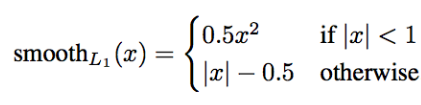
\includegraphics[width=0.5\textwidth]{smoothl1}
    \caption{Smooth L1 Loss Function}
    \label{fig:smoothl11}
\end{figure}
\indent

Loss functions are used to measure the difference between ground-truth 
values and the predicted values in machine learning problems. Loss 
functions can also be called error functions. Thus, the aim is to minimize 
the value of loss function during training to have a better detector. 
In object detection problems, loss functions are composed of two parts: 
regression difference and classification difference. Loss functions are 
the measure of difference between predicted regression box and 
ground-truth regression box and also, the difference between the correct 
class for object and the predicted class for object. These functions can 
vary based on design choices and different loss functions have different 
advantages and disadvantages. The most frequent used loss functions as 
following:
\begin{itemize}
    \item L1 Loss Function
    
    L1 loss function minimizes the absolute differences between the
    predicted value and ground-truth value.

    $$\sum_{i=1}^{n} (|y_t - y_p|)$$

    \item L2 Loss Function
    
    L2 loss function minimizes the squared differences between the 
    predicted value and ground-truth value.

    $$\sum_{i=1}^{n} (y_t - y_i)^{2}$$

    \item Smooth L1 Loss Function
    
    The function of smooth L1 loss function can be seen in the figure \ref{fig:smoothl11}.

    \item Cross-Entropy Loss Function

    $$\sum_{i=1}^{n} (y_t * \log (y_i))$$

\end{itemize}    
\indent

Since L1 loss function operates on the absolute values, it does not 
affected by outliers. Therefore, L1 is more robust to outliers. On the
other hand, L2 loss function operates on the squared values, therefore, 
L2 is not robust to outliers since outliers will cause a huge error value. 
However, if one analyzes and see there is not many outliers in data, then, 
using L2 loss function leads to a better training. Smooth L1 loss function is a 
combination of L1 and L2 loss functions. When absolute value of loss is small, it 
behaves similar to L2 loss but when absolute value of loss is high, it behaves 
similar to L1 loss. Thus, it shares the advantages of both loss functions. Cross-entropy 
loss function measures the performance of a classification. 
\end{document}